\begin{figure}[htbp]
	\centering
	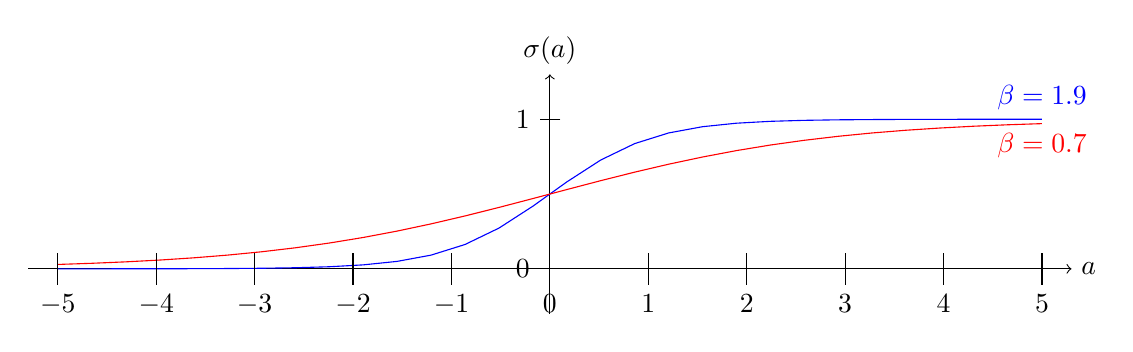
\begin{tikzpicture}[yscale=1.9,xscale=1.25]
		\def \xMin {-5};
		\def \xMax {5};
		\def \yMin {0};
		\def \yMax {1.};
		\draw[->] (\xMin - 0.3,0) -- (\xMax + 0.3,0) node[right] {$a$};
		\draw[->] (0,\yMin - 0.3) --(0,\yMax + 0.3) node[above] {$\sigma(a)$};
		\draw[domain=\xMin:\xMax,samples=30,variable=\x,blue]
			plot ({\x},{1 / (1 +  exp(-1.9*\x))}) node[above] {$\beta=1.9$};
		\draw[domain=\xMin:\xMax,samples=30,variable=\x,red]
			plot ({\x},{1 / (1 +  exp(-0.7*\x))}) node[below] {$\beta=0.7$};
		\foreach \tic in {\yMin,...,\yMax}
     	{
     		\draw[shift={(0,\tic)},color=black] (3pt,0pt) -- (-3pt,0pt) node[left] {$\tic$};
     	}
     	\foreach \tic in {\xMin,...,\xMax}
     	{
     		\draw[shift={(\tic,0)},color=black] (0pt,3pt) -- (0pt,-3pt) node[below] {$\tic$};
     	}
 
	\end{tikzpicture}
	\caption{Two variations of the sigmoid activation function}
	\label{fig:modified_sigmoid}
\end{figure}
